\section{Evaluation}
\label{sec:evaluation}

This section answers the research questions using the frozen results pack in \texttt{results/final\_pack/} and the report-ready imports under \texttt{report/figures/final\_pack/}.

\subsection{Experimental setup}
All experiments use the CIFAR-10 test set and a fixed index set of 10{,}000 images (indices 0--9{,}999). An image is considered \emph{eligible} if it is classified correctly by the clean model; this yields 9{,}213 eligible images. The threat model is black-box and restricted to a single-pixel perturbation: an adversarial example differs from the clean input at exactly one $(x,y)$ location and may change all three RGB channel values at that pixel.

The baseline attack is an untargeted one-pixel Differential Evolution (DE) search. Two guidance variants are evaluated for RQ2: (i) a fastprior variant that uses a fixed-budget multi-target DE configuration, and (ii) a responsibility-map-guided DE variant that uses a black-box saliency prior derived from RISE to bias pixel selection and mutation. Attacks are evaluated by image-wise success rate (ASR) on the eligible set and by query cost (number of model evaluations), summarised using medians over all trials and over successful trials.

For RQ1 and RQ2 explanation analysis, three explainers are computed: Grad-CAM, Integrated Gradients (IG), and RISE. Stability is measured on successful adversarial examples using IoU@10 (overlap of the top-$k$ salient pixels with $k=10$) and Spearman rank correlation $\rho$ between attribution maps before vs after the attack. Faithfulness is assessed via deletion AUC, reported for clean and adversarial inputs and as the difference (adversarial minus clean).

\subsection{RQ1: How do successful one-pixel attacks affect explanations?}

\paragraph{RQ1: Explanation stability under successful one-pixel attacks.}
RQ1 is evaluated on the successful untargeted adversarial subset, which contains 3{,}477 successful attacks drawn from the 9{,}213 eligible images in the 10{,}000-index evaluation set.
Across explainers, Integrated Gradients exhibits the highest stability, with mean IoU@10 of 0.485 and mean Spearman $\rho$ of 0.842.
Grad-CAM achieves mean IoU@10 of 0.326 and mean $\rho$ of 0.695, while RISE shows comparable IoU@10 (0.322) but substantially lower rank-stability (mean $\rho$ of 0.477).
Faithfulness measured by deletion AUC also deteriorates under successful attacks for all explainers: the mean change (adversarial minus clean) is negative for Grad-CAM (-0.173), IG (-0.060), and RISE (-0.165).
Overall, successful one-pixel perturbations are associated with reduced faithfulness and method-dependent explanation stability, with IG the most stable of the three evaluated explainers under this protocol.

\begin{figure}[t]
  \centering
  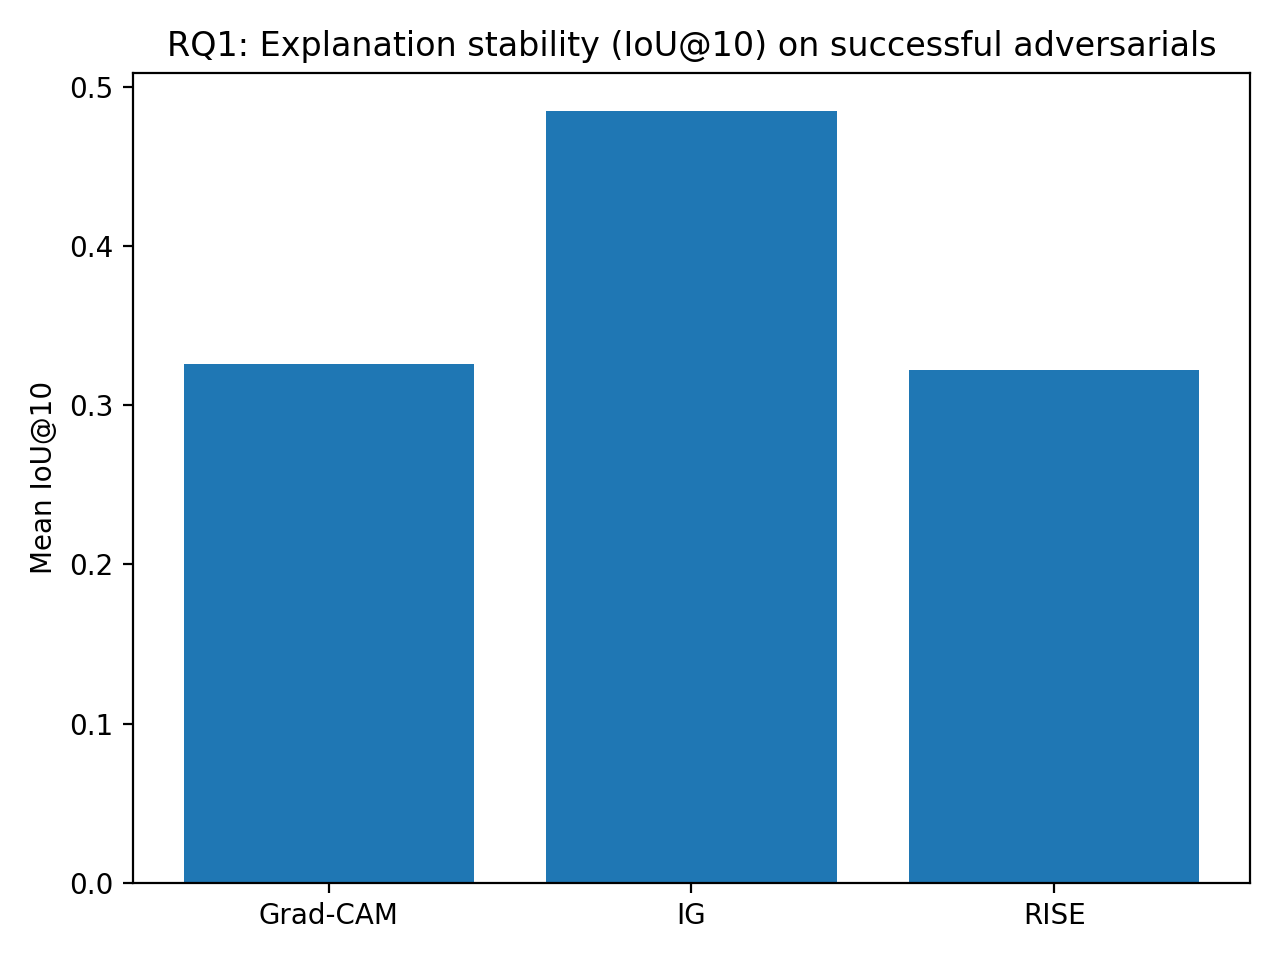
\includegraphics[width=0.85\linewidth]{figures/final_pack/rq1_iou10_adv_mean.png}
  \caption{RQ1: Mean IoU@10 on successful adversarial examples (higher indicates more stable explanations).}
  \label{fig:rq1_iou10}
\end{figure}

\begin{figure}[t]
  \centering
  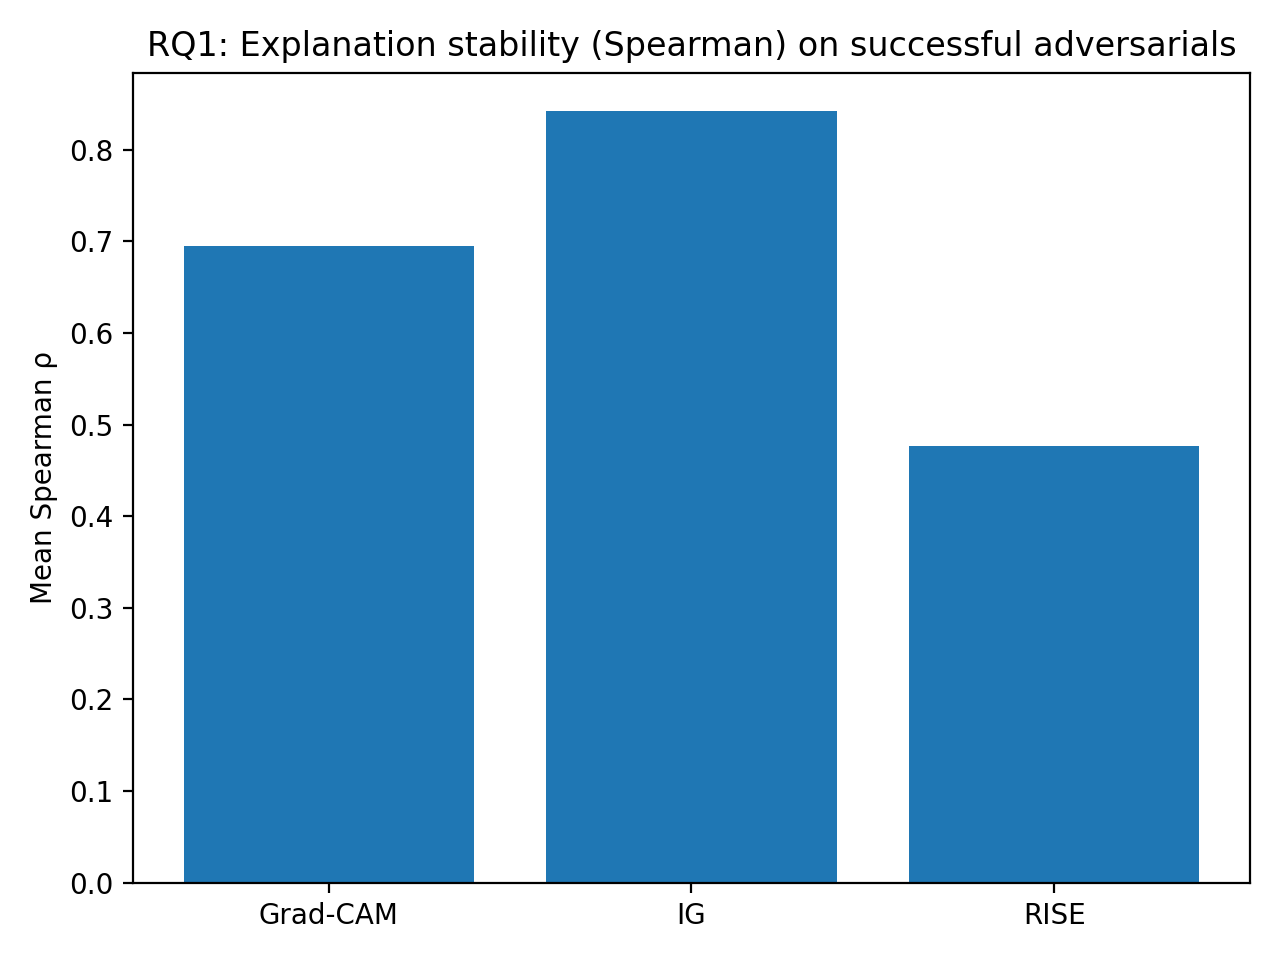
\includegraphics[width=0.85\linewidth]{figures/final_pack/rq1_rho_adv_mean.png}
  \caption{RQ1: Mean Spearman rank correlation on successful adversarial examples.}
  \label{fig:rq1_rho}
\end{figure}

\begin{figure}[t]
  \centering
  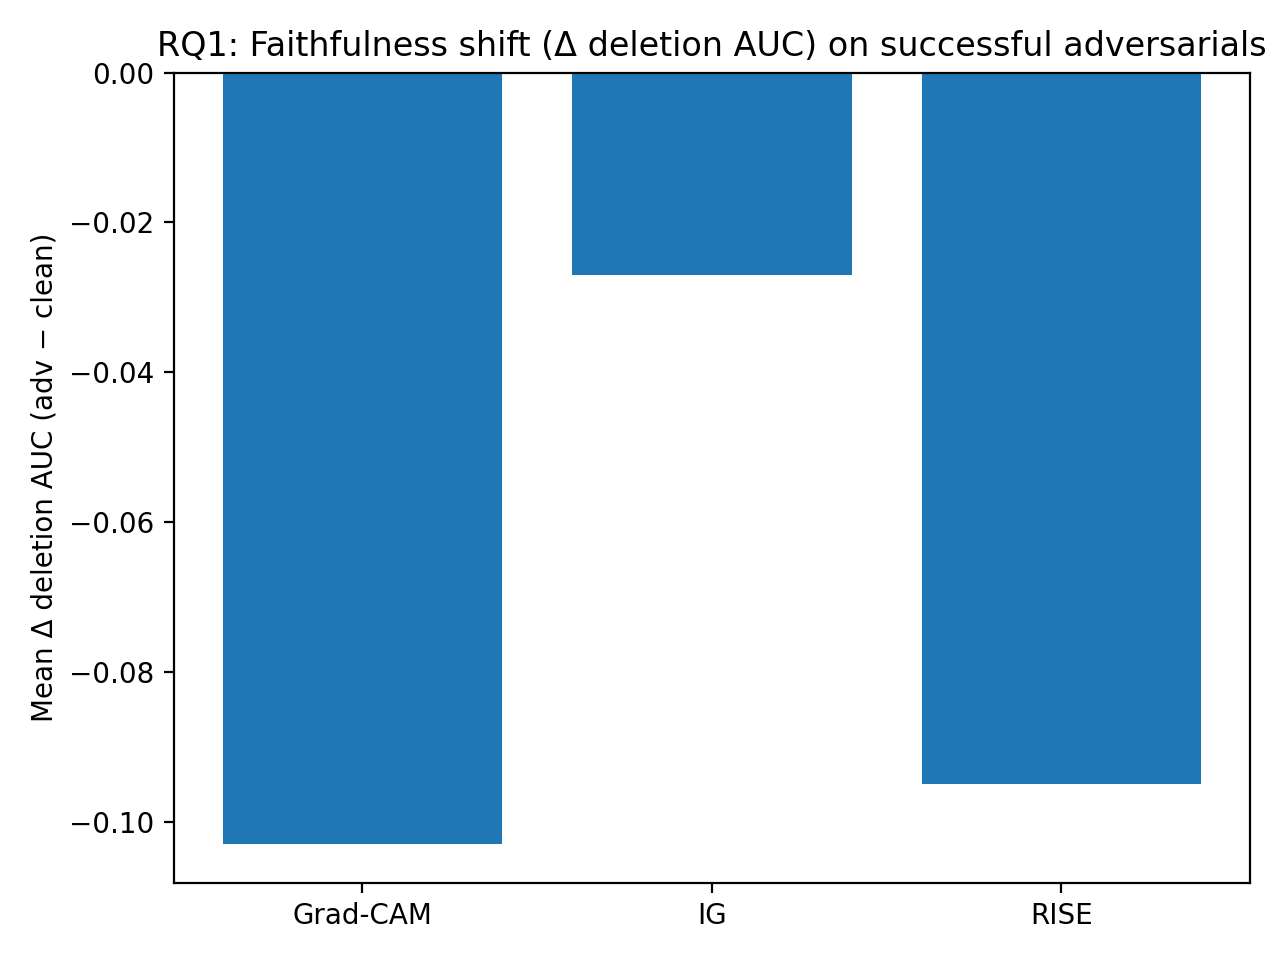
\includegraphics[width=0.85\linewidth]{figures/final_pack/rq1_del_auc_delta_mean.png}
  \caption{RQ1: Mean change in deletion AUC (adversarial minus clean) on successful adversarial examples.}
  \label{fig:rq1_delauc_delta}
\end{figure}

\subsection{RQ2: Can responsibility-map guidance improve one-pixel attacks?}

\subsubsection{Effectiveness and query cost}
\begin{table}[t]
\centering
\small
\caption{RQ2 attack outcomes on the eligible CIFAR-10 subset (9{,}213 images): image-wise success rate (ASR) and query cost.}
\label{tab:rq2_attack_summary}
\begin{tabular}{lrrrrr}
\toprule
Run & Eligible & Success & ASR & Median queries (succ) & Median queries (all) \\
\midrule
untargeted & 9,213 & 3,477 & 0.377 & 6,000 & 40,400 \\
fastprior & 9,213 & 1,310 & 0.142 & 70,848 & 70,848 \\
rise-guided & 9,213 & 3,477 & 0.377 & 6,400 & 40,400 \\
\bottomrule
\end{tabular}

\end{table}


\begin{figure}[t]
  \centering
  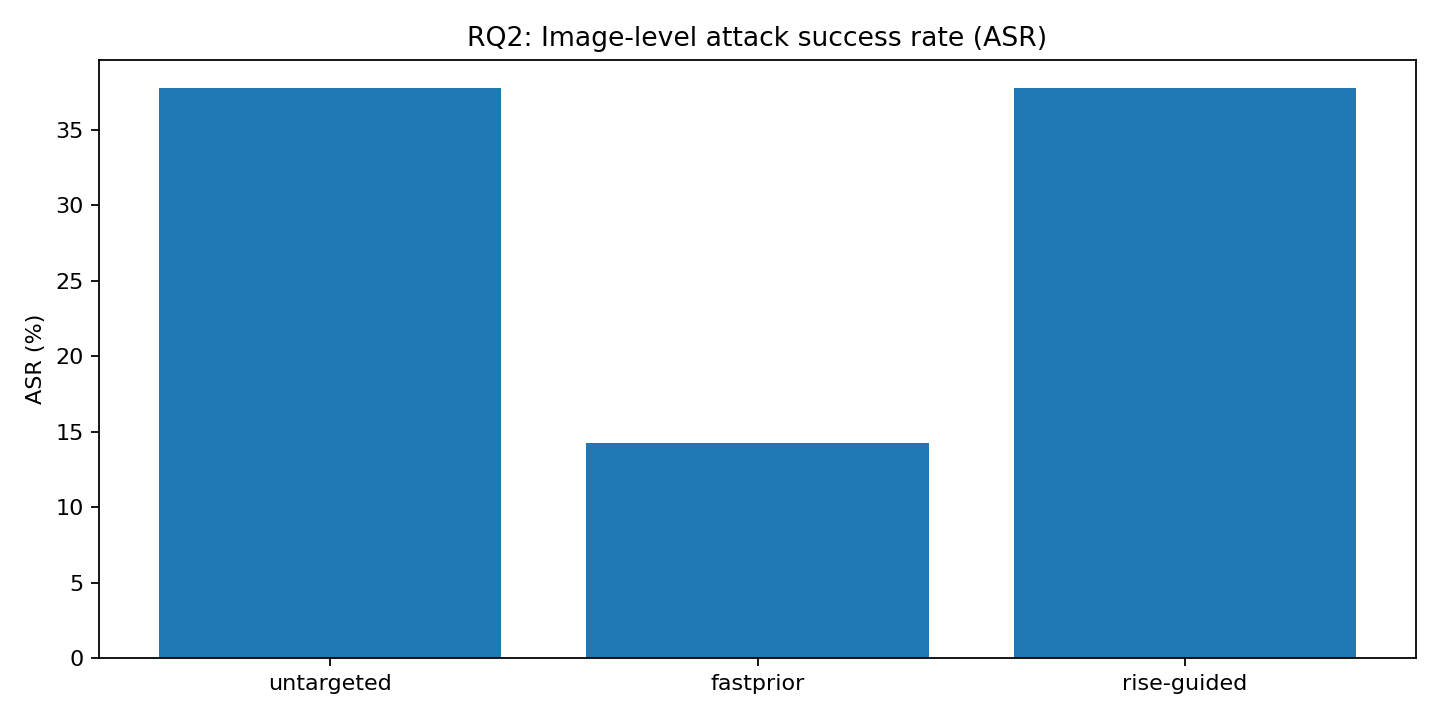
\includegraphics[width=0.85\linewidth]{figures/final_pack/rq2_asr_image_percent.png}
  \caption{Image-wise attack success rate (ASR) on the 9{,}213 eligible CIFAR-10 test images.}
  \label{fig:rq2_asr}
\end{figure}

\begin{figure}[t]
  \centering
  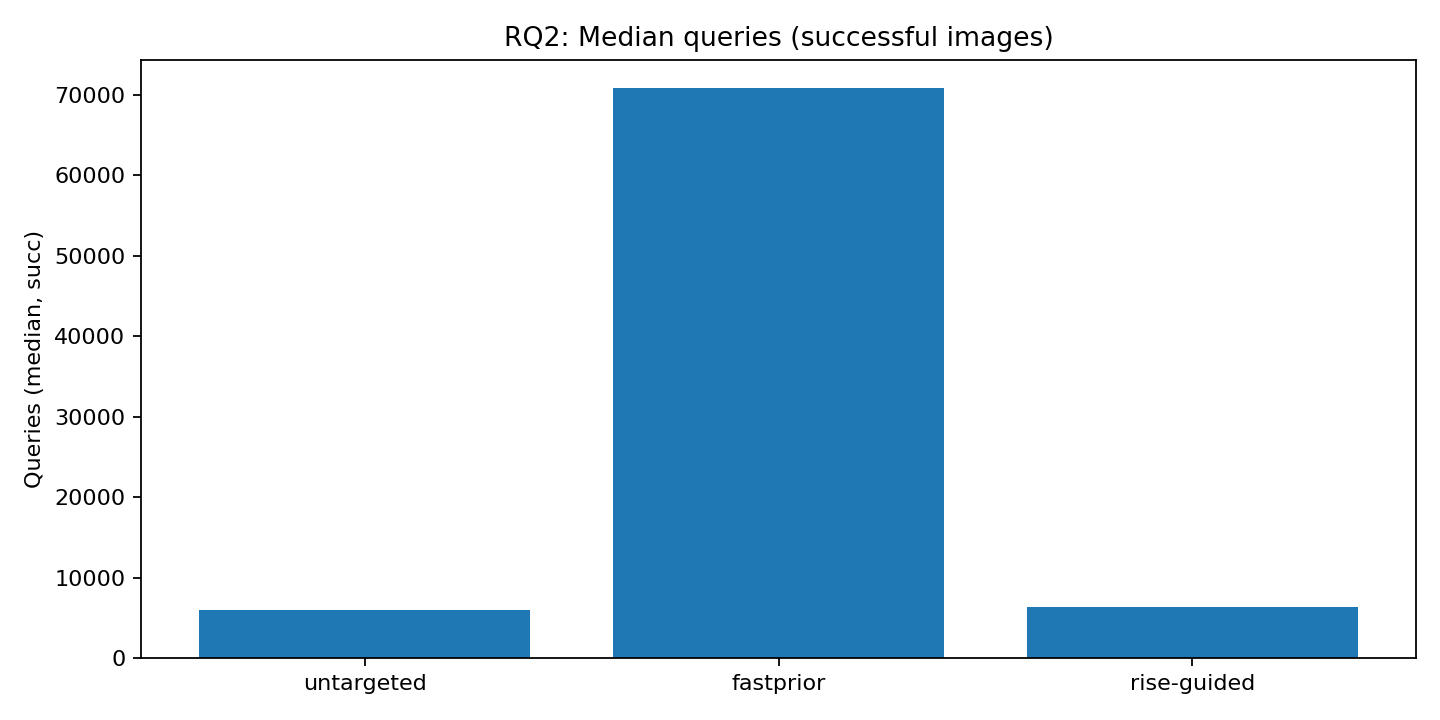
\includegraphics[width=0.85\linewidth]{figures/final_pack/rq2_queries_median_success.png}
  \caption{Median query cost among successful attacks (lower is better).}
  \label{fig:rq2_queries_succ}
\end{figure}

\paragraph{Effectiveness and query cost.}
Table~\ref{tab:rq2_attack_summary} and Figures~\ref{fig:rq2_asr}--\ref{fig:rq2_queries_succ} summarise the trade-off between image-wise success rate (ASR) and query cost on the 9{,}213 eligible CIFAR-10 test images.
The untargeted DE baseline achieves an ASR of 0.3774 (3{,}477/9{,}213), with median query cost 6{,}000 among successful attacks and 40{,}400 over all eligible images.
The fastprior variant reduces image-wise ASR to 0.1422 (1{,}310/9{,}213) and is substantially more expensive in this configuration, with median query cost 70{,}848 both overall and among successful images, reflecting its fixed-budget design.
At the target level, fastprior records 1{,}482 successful targets out of 82{,}917 target attempts (1.8\%), showing that it does find successful targets but converts these into successful images much less often than the untargeted baseline.
The RISE-guided variant achieves the same ASR as the unguided baseline (0.3774; 3{,}477/9{,}213) but changes the cost profile among successful attacks: the median successful query cost increases from 6{,}000 to 6{,}400, while the overall median remains 40{,}400.
Overall, the evaluated guidance strategies do not improve the headline success--cost frontier at 10k scale: fastprior trades image-wise success for stability, while simple RISE guidance preserves ASR but does not reduce query cost.

\subsubsection{Explanation stability among successful adversarials}
\begin{table}
\begingroup
\hbadness=10000
\hfuzz=100pt
\setlength{\emergencystretch}{2em}
\sloppy
[t]
\centering
\scriptsize
\setlength{\tabcolsep}{3pt}
\renewcommand{\arraystretch}{1.15}
\small
\resizebox{0.92\linewidth}{!}{%
\begin{minipage}{\linewidth}
\caption{RQ2 explanation stability on successful adversarial examples (means). Higher IoU@10 and Spearman indicate more stable explanations.}
\label{tab:rq2_stability_means}
\begin{tabular}{lrrrrrr}
\toprule
Run & IoU@10 GC & IoU@10 IG & IoU@10 RISE & Spearman GC & Spearman IG & Spearman RISE \\
\midrule
untargeted & 0.326 & 0.485 & 0.322 & 0.695 & 0.842 & 0.477 \\
fastprior & 0.517 & 0.532 & 0.367 & 0.839 & 0.866 & 0.525 \\
rise-guided & 0.325 & 0.484 & 0.296 & 0.693 & 0.842 & 0.445 \\
\bottomrule
\end{tabular}

\end{minipage}}
\endgroup
\end{table}

\begin{table}[t]
\centering
\small
\setlength{\tabcolsep}{4pt}
\renewcommand{\arraystretch}{1.15}
\caption{RQ2 faithfulness shift under attack: mean change in deletion AUC (adversarial minus clean) on successful adversarial examples. More negative indicates a larger drop.}
\label{tab:rq2_del_delta}
\begin{tabular}{lrrr}
\toprule
Run & $\Delta$DelAUC GC & $\Delta$DelAUC IG & $\Delta$DelAUC RISE \\
\midrule
untargeted & -0.173 & -0.060 & -0.165 \\
fastprior & -0.148 & -0.069 & -0.148 \\
rise-guided & -0.173 & -0.060 & -0.159 \\
\bottomrule
\end{tabular}
\end{table}


\begin{figure}[t]
  \centering
  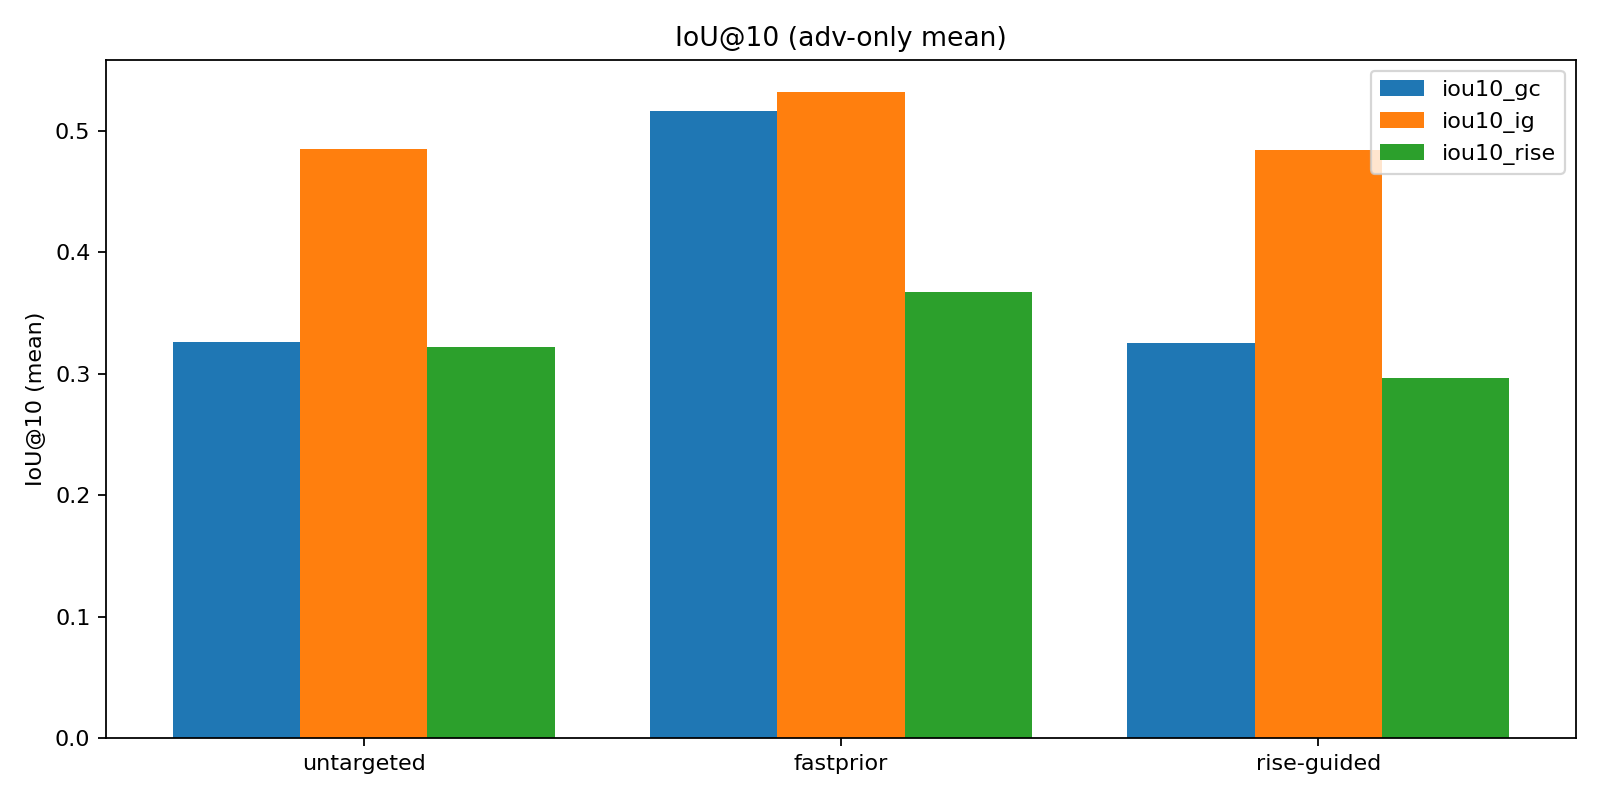
\includegraphics[width=0.85\linewidth]{figures/final_pack/rq2_iou10_adv_mean.png}
  \caption{Mean IoU@10 of explanation maps on successful adversarial examples (higher indicates more stable explanations).}
  \label{fig:rq2_iou10}
\end{figure}

\begin{figure}[t]
  \centering
  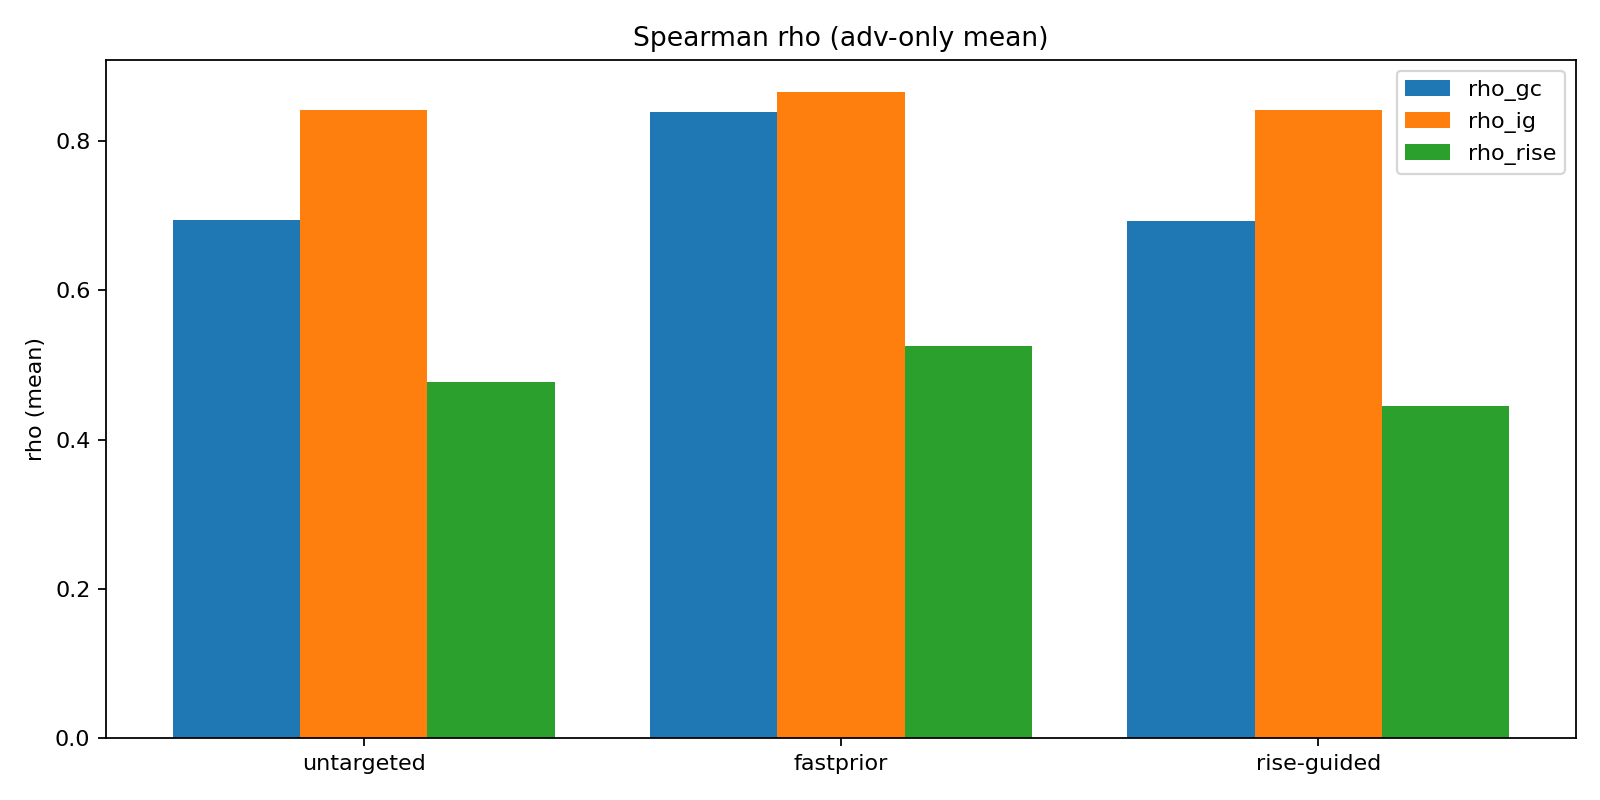
\includegraphics[width=0.85\linewidth]{figures/final_pack/rq2_rho_adv_mean.png}
  \caption{Mean Spearman rank correlation of attribution values on successful adversarial examples.}
  \label{fig:rq2_rho}
\end{figure}

\begin{figure}[t]
  \centering
  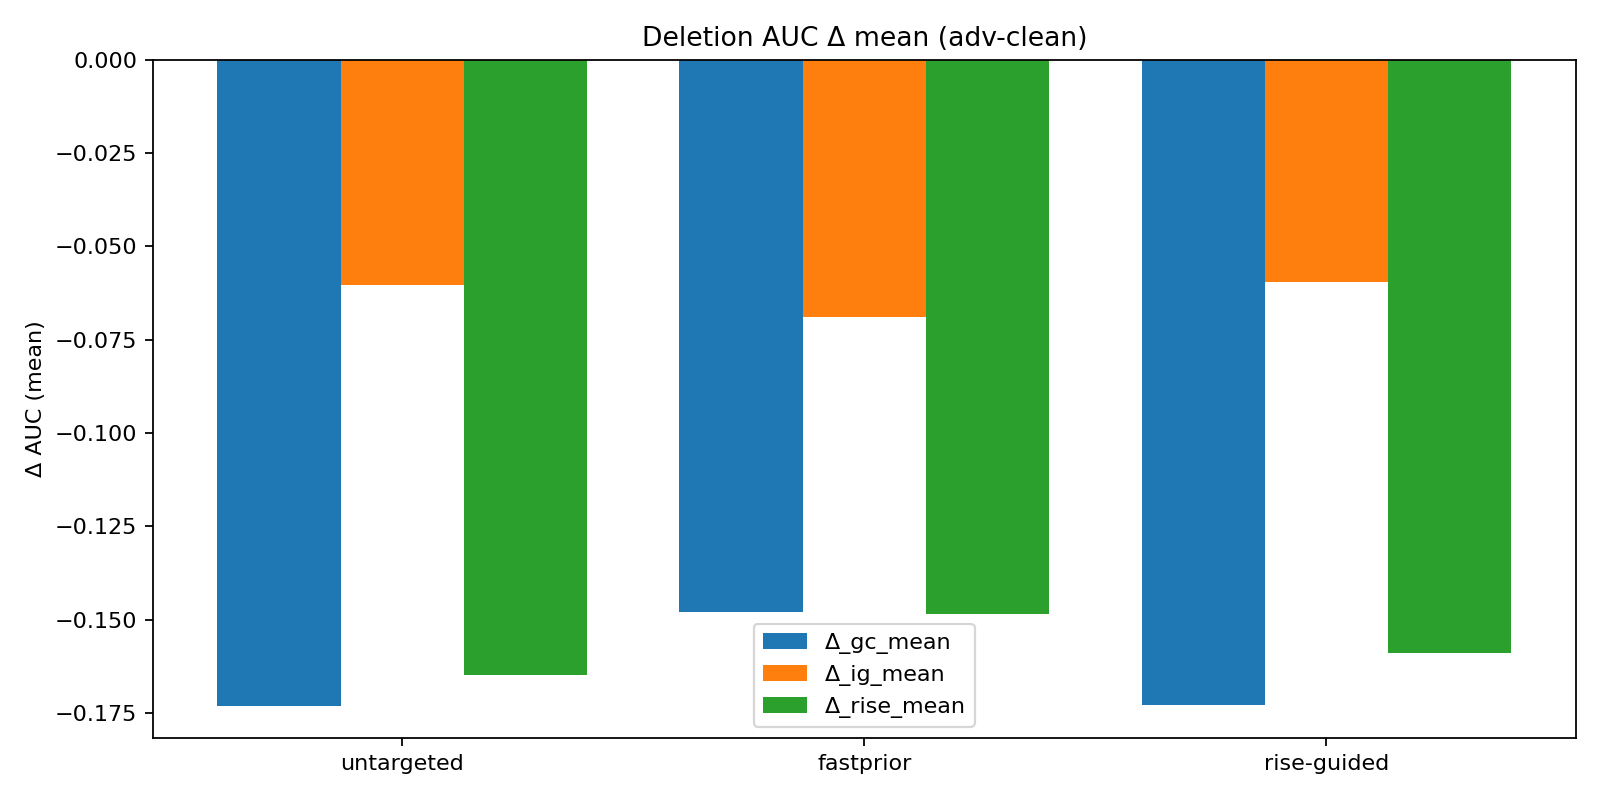
\includegraphics[width=0.85\linewidth]{figures/final_pack/rq2_del_auc_delta_mean.png}
  \caption{Mean change in deletion AUC (adversarial minus clean) on successful adversarial examples.}
  \label{fig:rq2_delauc_delta}
\end{figure}

\paragraph{Explanation stability among successful adversarials.}
Table~\ref{tab:rq2_stability_means}, Table~\ref{tab:rq2_del_delta}, and Figures~\ref{fig:rq2_iou10}--\ref{fig:rq2_delauc_delta} compare explanation stability and faithfulness metrics computed on successful adversarial examples.
Across all runs, Integrated Gradients exhibits the highest rank-stability, with mean Spearman $\rho$ 0.842 for untargeted, 0.866 for fastprior, and 0.842 for RISE-guided.
Comparing untargeted vs RISE-guided successes, Grad-CAM and IG are almost unchanged (for example, IoU@10 for Grad-CAM is 0.326 vs 0.325, and Spearman for IG is 0.842 vs 0.842), whereas RISE stability decreases under guidance (IoU@10: 0.322 to 0.296; Spearman: 0.477 to 0.445).
Fastprior successful cases are more stable across all three explainers (IoU@10 0.517/0.532/0.367 and Spearman 0.839/0.866/0.525 for Grad-CAM/IG/RISE), but this improvement comes together with much lower image-wise ASR and much higher query cost.
Deletion-based faithfulness degrades under successful attacks for all runs and methods, with negative mean $\Delta$ deletion AUC throughout: untargeted (-0.173, -0.060, -0.165), fastprior (-0.148, -0.069, -0.148), and RISE-guided (-0.173, -0.060, -0.159) for Grad-CAM, IG, and RISE respectively.
These results suggest that guidance changes the composition of successful adversarial examples rather than uniformly improving attack quality: some guided successes are more explanation-stable, but this does not translate into a better overall success--cost trade-off.

\subsection{Discussion and limitations}
Two clear themes emerge.
First, explanation behaviour under successful one-pixel attacks is method-dependent: IG is consistently more stable than Grad-CAM and RISE, while all explainers show reduced deletion-based faithfulness on successful adversarial examples.
Second, responsibility-map guidance changes trade-offs rather than uniformly improving outcomes: fastprior produces more stable successful cases but at much lower image-wise success and much higher cost, while RISE-guided DE preserves headline ASR but does not improve efficiency and reduces RISE-based stability.

These results are conditioned on the specific threat model (single-pixel, black-box) and the chosen model and dataset.
The fastprior configuration uses a fixed budget, which makes its query cost less comparable to adaptive stopping strategies.
Explanation metrics are computed only on successful adversarial examples and therefore reflect both explanation sensitivity and the changed composition of successful cases under each attack configuration.
Finally, while the results are frozen and reproducible via the provided scripts and final results pack, broader generalisation to other architectures, datasets, or multi-pixel perturbations remains outside the scope of this evaluation.
